\chapter{On Graphs}
\section{What is a Graph?}
\lettrine[lines=4]{G}{raphs}, in their elementary form, are a pair of sets: $V$ (\textbf{Vertices}) and $E$ (\textbf{Edges}) such that $V \neq \emptyset$ ($V$ cannot be empty), and $\forall e \in E, e = \{v_i, v_j\}, v_i, v_j \in V$ (every edge in $E$ is a pairwise subset of vertices $v_i$ and $v_j$ in $V$). Here is an example of a very simple graph:

\begin{center}
    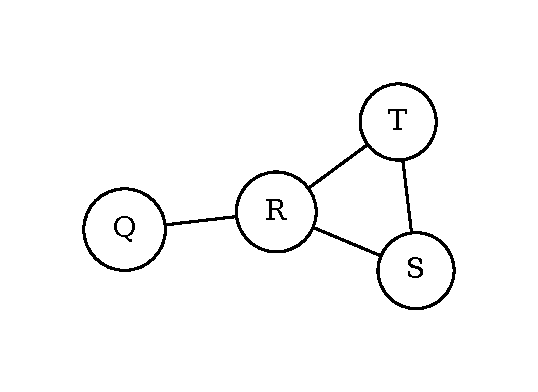
\includegraphics[width=0.5\textwidth]{Chapter1/graph.pdf}
\end{center}

In this graph, our vertex set is $V = \{Q, R, S, T\}$, and our edge set is $E = \big\{\{Q, R\}. \{R, S\}, \{R, T\}, \{S,T\}\big\}$.

Other names for Vertices are \textbf{nodes} or \textbf{points}. Other names for edges are \textbf{links} or \textbf{lines}. When we want to refer to the vertex set of a specific graph $G$, we will denote it as $V(G)$. Similarly, we will denote the edge set as $E(G)$.
\section{Why do we care about Graphs?}
Graphs can be used to model many real world problems, or theoretical ideas. For example, graphs can be used to represent relationships between different objects or groups. They are useful for visualizing data, such as social media connections, or network topology. Additionally, a more practical use is for mapping routes from one location to another, much like the GPS on your phone.

As for more theoretical uses, graphs can represent other structural relationships. Tree structures are a type of graph, as are flow diagrams or DFAs/NFAs from Computation Theory. Perhaps one of their more important uses is in determining where problems fit in P vs. NP.

\section{On Different Types of Graphs}
\subsection{Multigraphs}
A \textbf{multigraph} is a pair of sets $(V, E)$ such that $V \neq \emptyset$, and $E$ is a finite family of unordered pairs of $V$. That is to say, edges are not necessarily unique subsets, and do not have order. Thus, multigraphs allow for loops from one vertex to itself. Here is an example of a multigraph:

\begin{center}
    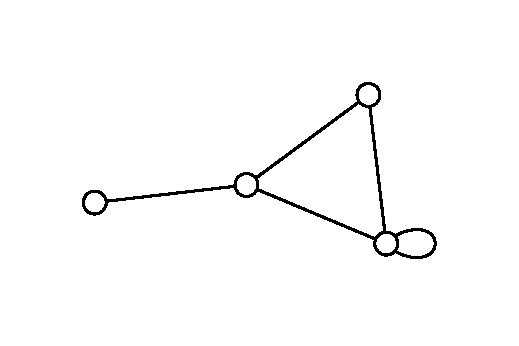
\includegraphics[width=0.5\textwidth]{Chapter1/multigraph.pdf}
\end{center}

Because multigraphs are unordered, then an edge $(a, b)$ would be the same as $(b, a)$. But what if we only want an edge in one direction but not the other?
\subsection{Digraphs}
A \textbf{digraph} is a pair of sets $(V, E)$ such that $V \neq \emptyset$, and $E$ is a set of ordered pairs of elements in $V$. Informally, we say that a digraph is a directed graph, where we annotate each edge with an arrow to mark the direction it flows. Here is an example of a digraph:

\begin{center}
    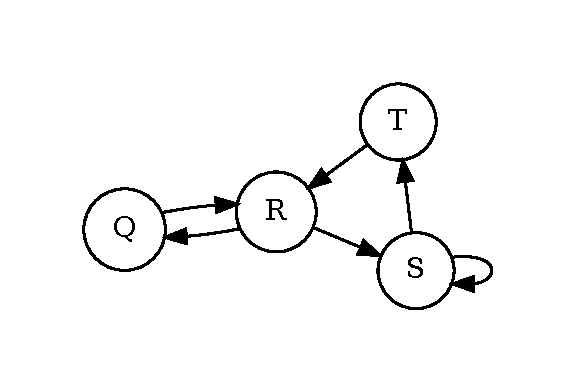
\includegraphics[width=0.5\textwidth]{Chapter1/digraph.pdf}
\end{center}

\section{On Vertices and Edges}
There is a lot to be said of the mathematics of graphs, but before we can establish such mathematics, we must first establish some essential definitions. Let $G$ be a graph with vertex set $V$ and edge set $E$. Let $u, v, w \in V$ be vertices of $G$.
\begin{description}
    \item[Join:] If $\{u, v\} \in E$, then $u$ is said to \textbf{join} $v$.
    \item[Adjacent:] $u$ and $v$ are said to be \textbf{adjacent} if $\{u, v\} \in E$. Similarly, if $\{u, v\}, \{u, w\} \in E$, then $\{u, v\}$ and $\{u, w\}$ are said to be \textbf{adjacent}.
    \item[Incident:] If $\{u, v\} \in E$, then $u$ and $v$ are said to be \textbf{incident} to $\{u, v\}$. Similarly, if $\{u, v\}, \{u, w\} \in E$, then $\{u, v\}$ and $\{u, w\}$ are said to be \textbf{incident} to $u$.
    \item[Degree:] The \textbf{degree} of a vertex, denoted deg($v$) or $\rho(v)$, is the number of edges incident to $v$.
    \item[Isolated:] If deg($v$) = 0, then we say $v$ is an \textbf{isolated} vertex.
    \item[Pendant:] If deg($v$) = 1, then we say $v$ is a \textbf{pendant} vertex.
\end{description}
These are a lot of formal definitions, but they will be useful when classifying different graphs and discussing their structures and properties. Informally, we say two edges are adjacent if they share a vertex, and two vertices are adjacent if they share an edge. Similarly, we say that two edges are incident to a vertex if they share that vertex, and two vertices are incident to an edge if they share that edge. 

\section{On Isomorphisms}
The term \emph{isomorphic} has its roots in Greek, \emph{iso-} meaning same, and \emph{morphic} referring to form or shape. We say that two graphs are \textbf{isomorphic} if they have this ``same shape'' property, but what does that mean?

Mathematically, we say that the graph $G_1$ is \textbf{isomorphic} to the graph $G_2$, denoted $G_1 \sim G_2$, if there is a one-to-one correspondence between the vertices $V_1$ of $G_1$ and the vertices $V_2$ of $G_2$ that preserves adjacencies. This is a mapping $f$ from $G_1$ to $G_2$ defined as follows:
\begin{center}
    $f : G_1 \mapsto G_2$ such that $\forall \{v_i, v_j\} \in E(G_1), \{f(v_i), f(v_j)\} \in E(G_2)$
\end{center}
This may look like a lot of intimidating gibberish, but it represents the idea of preserving the edges between two vertices in $G_1$ after mapping them to $G_2$. For example, the following graphs are isomorphic:
\begin{center}
    \includegraphics[width=0.4\textwidth]{Chapter1/isomorphicA.pdf} % Compile isomorphic.dot with neato
    \includegraphics[width=0.4\textwidth]{Chapter1/isomorphicB.pdf} % Compile isomorphic.dot with circo
\end{center}
Isomorphisms are a mapping, and thus have certain propoerties that allow us to classify them with other mappings. Let $G_1, G_2,$ and $G_3$ be graphs. Isomorphisms are what we call an equivalence relation, as the following three propoerties hold:
\begin{description}
    \item[Reflexive:] $G_1 \sim G_1$
    \item[Symmetric:] If $G_1 \sim G_2$, then $G_2 \sim G_1$
    \item[Transitive:] If $G_1 \sim G_2$ and $G_2 \sim G_3$, then $G_1 \sim G_3$
\end{description}

\subsection{The Handshaking Lemma}
We are now armed with enough information to decipher some information hidden in the graphs we deal with. The first of these is called the Handshaking Lemma. Let's tackle this proof:

\begin{lemma}[The Handshaking Lemma]
    Let $G$ be a graph. Then the number of vertices with odd degree is even.
\end{lemma}
\begin{proof}
    Let $V = \{v_1, v_2, \ldots, v_n\}$ be the vertices of $G$. The the sum of the degrees,
    \begin{equation*}
        \sum_{i=1}^n \text{deg}(v_i) = 2m, m \in \mathbb{Z},
    \end{equation*}
    is even, since each edge is counted twice (convince yourself that this must be true, if you don't understand). Now, if we were to remove all vertices of even degree, then we would be removing an even number of edges from this sum. This leaves us with
    \begin{equation*}
        \sum_{odd~degrees}^n \text{deg}(v_i) = 2k, k \in \mathbb{Z},
    \end{equation*}
    which is even. Now, the only way for the sum of odd numbers to be even is for there to be an even number of those odds. Thus, we must have an even number of odd degree vertices in $G$.
\end{proof}
\section{On Special Kinds of Graphs}
We've talked a lot about the different aspects of graphs, but now let's use this information to actually classify different kinds of graphs, starting with the \textbf{null graph}. the null graph is a graph with $n$ vertices but no edges, and is denoted as $N_n$.

A \textbf{regular graph} is a graph $G$ with $n$ vertices whose vertices all have the same degree, and we say such a graph is regular of degree $r < n$.

A \textbf{complete graph} is a graph $G$ with $n$ vertices that is regular of degree $n-1$. We denote such a graph by $K_n$. The total number of edges in the complete graph $K_n$ is given by summing the number of edges: 
\begin{equation*}
    \sum_{i=1}^{n-1} i = \frac{(n-1)(n-2)}{2}
\end{equation*}

A \textbf{bipartite graph} is a graph with vertex set $V = V_1 \cup V_2$ where $V_1 \cap V_2 = \emptyset$ and $\forall v_i, v_j \in V_1$ and $v_m, v_n \in V_2$, $(v_i, v_j), (v_m, v_n) \not\in E$. This is another way to say that the vertices of a bipartite graph $G$ can be divided into two sets there all edges in $G$ only go between both sets - neither set of vertices has two vertices which make an edge. A complete bipartite graph is denoted $K_{m, n}$, with two sets containing $m$ and $n$ vertices, with all vertices in one set connecting to all the vertices of the other. Here is an example of a bipartite graph, $K_{3, 3}$:
\begin{center}
    \includegraphics[width=0.3\textwidth]{Chapter1/isomorphicB.pdf}
\end{center}

A \textbf{subgraph} of $G = (V, E)$ has the vertex set $H$ and the edge set $F$, where $H \subseteq V$ and $F \subseteq E$, but only the edges of $E$ which correspond to the vertices in $H$ can be in $F$.

\section{On the Storage of Graphs}
We've talked a lot about graphs and their theories and applications, but how exactly do we represent graphs in a computer? The idea that a graph defines a set of relations in important, so the natural way to consider this is some sort of data structure with nodes which point to their adjacent neighbors. This certainly is an intuitive way to consider this, but examining them mathematically will make our lives easier in the future.

Consider the following graph:
\begin{center}
    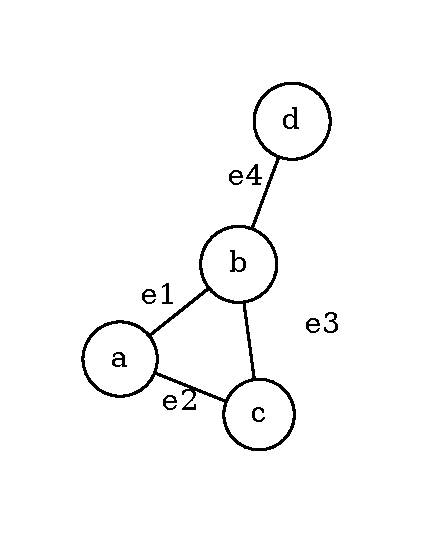
\includegraphics[width=0.5\textwidth]{Chapter1/mat.pdf}
\end{center}
We can store this in what's called an \textbf{Adjacency Matrix}, a matrix where each row and column represents a particular vertex in the graph, and entries in the matrix signify that two vertices share an edge. The adjacency matrix for the given graph is:
\begin{center}
    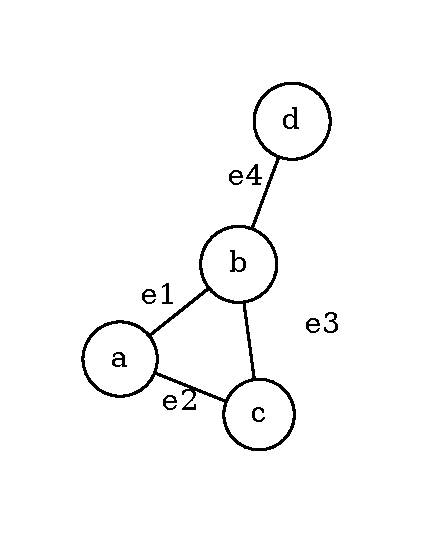
\includegraphics[width=0.4\textwidth]{Chapter1/mat.pdf} $\bordermatrix{~ & a & b & c & d \cr
                                                                           a & 0 & 1 & 1 & 0 \cr
                                                                           b & 1 & 0 & 1 & 1 \cr
                                                                           c & 1 & 1 & 0 & 0 \cr
                                                                           d & 0 & 1 & 0 & 0 }$
\end{center}
We usually denote an adjacency matrix $[A_{i, j}]$, where a 1 in entry $a_{i, j}$ identifies that vertices $i$ and $j$ share an edge, and a 0 means that they don't. While adjacency matrices for a graph with $n$ vertices occupies $n^2$ space, they do provide constant lookup time to see if two vertices share an edge.

We also have an \textbf{Incidence Matrix}, which tells us if an edge and a vertex are incident. The incidence matrix for the graph above is:
\begin{center}
    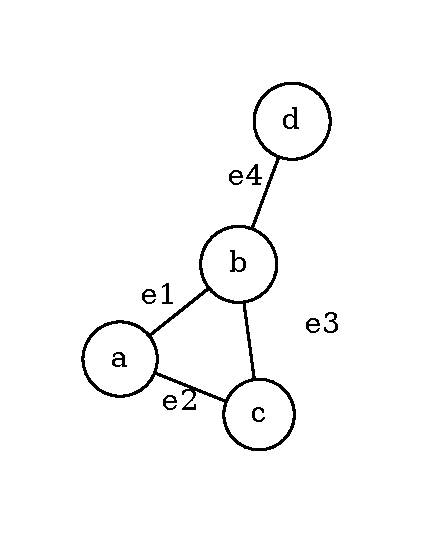
\includegraphics[width=0.4\textwidth]{Chapter1/mat.pdf} $\bordermatrix{~ & e_1 & e_2 & e_3 & e_4 \cr
                                                                           a & 1 & 1 & 0 & 0 \cr
                                                                           b & 1 & 0 & 1 & 1 \cr
                                                                           c & 0 & 1 & 1 & 0 \cr
                                                                           d & 0 & 0 & 0 & 1 }$
\end{center}
It might be preferable to use the adjacency matrix for the symmetry along the main diagonal of the matrix. 

% \bibliographystyle{acm}
% \bibliography{bibliography}